\chapter{MATERIALS AND METHODS}

\section{Experimental Data Preparation}
\subsection{Data Acquisition}
Extracellular metabolomics data is obtained from Cakar's Lab \cite{arslan2018physiological}. \hl{Missing sentence: What they did was...} Briefly, ethyl methane sulfonate (EMS) mutagenesis was performed on the prototrophic \emph{Saccharomyces cerevisiae} strain CEN.PK 113-7D (MATa, MAL2-8c, SUC2) to increase the genetic diversity as an evolutionary engineering selection strategy. Cells were inoculated in 2\% Yeast Minimal Media (YMM), and the extracellular concentrations of glucose, ethanol, glycerol and acetate were measured at different time points. OD\textsubscript{600} values were determined by a spectrophotometer. Additionally, cell dry weight analysis was conducted to determine biomass production. Acquired extracellular metabolite concentrations, OD\textsubscript{600} values and dry weights of the reference strain (without mutagenesis) were used in this study are collected in Table \ref{table:experimental_data} and Table \ref{table:experimental_OD600s_and_growths}.


\begin{table}[H]
\caption[Measurements of extracellular concentrations \cite{surmeli2019evolutionary}]{Measurements of extracellular concentrations \cite{surmeli2019evolutionary}.}
\begin{center}
\begin{tabular}{|c|c|c|c|c|}
   \hline
  \textbf{Time(h)} & \textbf{Glucose(g/L)} & \textbf{Ethanol(g/L)} & \textbf{Glycerol(g/L)} & \textbf{Acetate(g/L)} \\
    \hline
  0                 & 19.99            & 0                & 0                 & 1.08             \\
  3                 & 17.98            & 0.58             & 0.02              & 1.24             \\
  6                 & 15.85            & 1.2              & 0.06              & 1.16             \\
  9                 & 12.21            & 3.39             & 0.18              & 1.37             \\
  12                & 9.18             & 7.97             & 0.61              & 2.45             \\
  15                & 0.4              & 8.17             & 0.69              & 2.46             \\
  27                & 0                & 8.28             & 0.76              & 2.6              \\
  46                & 0                & 8                & 0.77              & 2.45             \\
  50                & 0                & 6.62             & 0.64              & 2.02             \\
  54                & 0                & 5.74             & 0.55              & 1.73             \\
  58                & 0                & 5.46             & 0.54              & 1.74             \\
  72                & 0                & 3.72             & 0.49              & 1.33            \\
   \hline
\end{tabular}
\label{table:experimental_data}
\end{center}
\end{table}

\begin{table}[H]
\caption[Measured OD\textsubscript{600} and cell dry weight values of reference strain \cite{surmeli2019evolutionary}]{Measured OD\textsubscript{600} and cell dry weight values of reference strain \cite{surmeli2019evolutionary}.}
\begin{center}
  \begin{tabular}{|c|c|c|c|}
 \hline
  \textbf{Time (h)} & \textbf{OD600} & \textbf{ln(OD600)} & \textbf{Cell DW (g/L)} \\
  \hline
  0                 & 0.21           & -1.560647748       & -                      \\
  3                 & 0.53           & -0.634878272       & -                      \\
  6                 & 1.76           & 0.565313809        & 0.9                    \\
  7.5               & 2.66           & 0.978326123        & -                      \\
  9                 & 4.46           & 1.495148766        & 1.9                    \\
  12                & 5.31           & 1.669591835        & -                      \\
  15                & 5.88           & 1.771556762        & -                      \\
  18                & 5.83           & 1.763017           & 2.32                   \\
  21                & 6.07           & 1.803358605        & -                      \\
  24                & 5.87           & 1.769854634        & -                      \\
  30                & 6.14           & 1.814824742        & 2.26                   \\
  40                & 6.44           & 1.86252854         & -                      \\
  46                & 6.36           & 1.850028377        & -                      \\
  50                & 6.3            & 1.840549633        & -                      \\
  54                & 6.55           & 1.87946505         & -                      \\
  63                & 6.54           & 1.877937165        & -                      \\
  67                & 6.88           & 1.928618652        & -                      \\
  72                & 6.97           & 1.941615225        & 2.66                  \\
   \hline
  \end{tabular}
\label{table:experimental_OD600s_and_growths}
\end{center}
\end{table}

\subsection{Determination of Rates}
As the slope of the curve of lnOD\textsubscript{600} as a function of time gives the growth rates, natural logarithm of OD\textsubscript{600} values were calculated to obtain specific growth rates by using the equation \ref{eq:growthrates}.
  \begin{equation}
      \ \mu = \frac{\Delta \ln{OD_{600}}}{\Delta t}
      \label{eq:growthrates}
  \end{equation}

In order to determine uptake and secretion rates of the metabolites, the steady-state assumption is applied in 3 hours intervals as they are the shortest measured intervals. Missing data on cell dry weights are estimated from the OD\textsubscript{600} values, and these cell dry weight data is used to calculate fluxes (in the unit of mmol/gDWh). Measurement of the cell dry weight at the 3rd hour was crucial for the steady-state assumption, however this data was missing. Curve trend of the OD600 values is used as a guide to estimate cell dry weight (Figure \ref{fig:GrowthGraphs}) \hl{Missing method: Estimation approach, similar to regression/curve fitting etc...}. Calculated flux values can be found in the Table \ref{table:calculated_fluxes}.

\begin{figure}[htbp]
\begin{center}
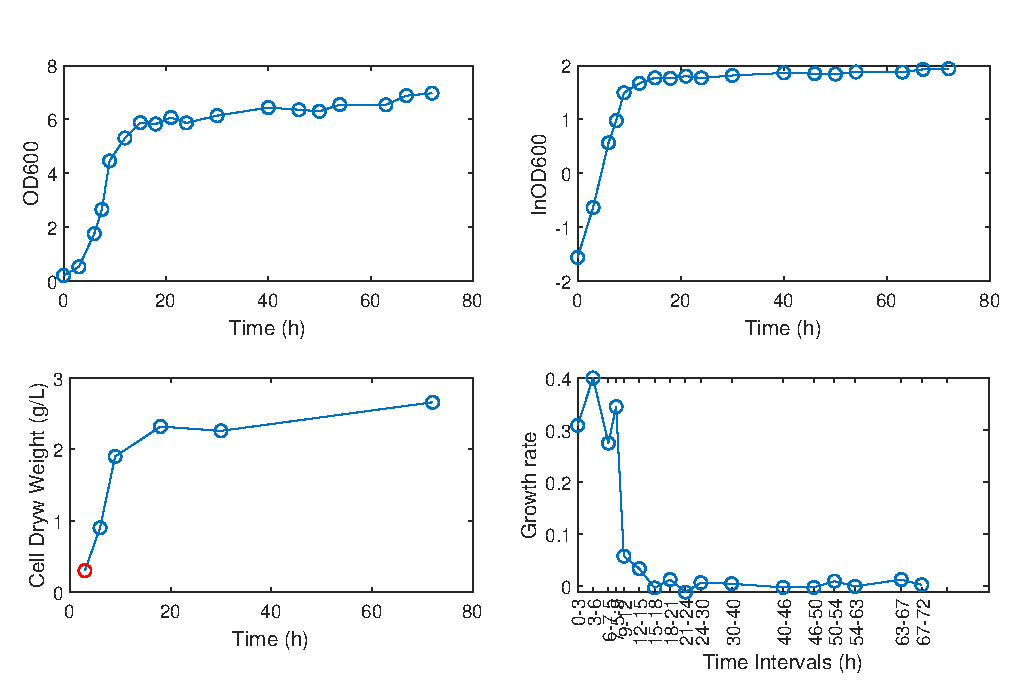
\includegraphics[width=1\columnwidth]{GrowthGraphsSmall.eps}
\end{center}
\caption{OD\textsubscript{600}, lnOD\textsubscript{600}, cell dry weights and growth rates graphs. Estimated missing cell dry weight data is shown in red color.}
\vskip\baselineskip % Leave a vertical skip below the figure
\label{fig:GrowthGraphs}
\end{figure}

\begin{table}[thbp]
\vskip\baselineskip
\caption[Calculated flux values]{Calculated flux values.}
\begin{center}
  \begin{tabular}{cccccc}
  \multicolumn{1}{l}{\textbf{Time}} & \multicolumn{4}{c}{\textbf{Metabolite fluxes in mmol/gDWh}}                & \textbf{Growth h-1} \\
  \textbf{}                         & \textbf{Glucose} & \textbf{Ethanol} & \textbf{Glycerol} & \textbf{Acetate} & \textbf{Biomass}    \\
  0-3                               & -12.3963884      & 13.98837518      & 0.24131           & 2.960496         & 0.30859             \\
  3-6                               & -4.378823762     & 4.984363569      & 0.160873          & -0.49342         & 0.400064
  \end{tabular}
\label{table:calculated_fluxes}
\end{center}
\end{table}


\section{Model Selection}
iAN50, a stoichiometric model of intermediary metabolism including glycolysis, the pentose phosphate pathway, anaerobic excretion, citric acid cycle (TCA cycle), oxidative phosphorylation, and uptake pathways for galactose, ethanol and acetate is used to simulate \cite{nilsson2016metabolic}.

\section{Flux Balance Analysis}
\section{Simulation of Batch Conditions}
